\section{D-Reducibility}
\label{sec:dreduce}

\subsection{Definitions}

The proof of the four-color theorem consists of proving that every graph has a certain subgraph that can be reduced to a smaller graph. So far, we have proven reducibility only for graphs containing the rings $R_4$ and $R_5$. The graphs that we we're left with we called Birkhoff graphs.

Since Birkhoff graphs already contain a lot of structure and information, our hopes are that every such Birkhoff graph contains \textbf{at least one subgraph of a finite set of reducible subgraphs}. We will call these subgraphs \textit{configurations}.

\begin{definition}
    A configuration is a triangulation where the outer vertices form a ring $R_n$ of size $n \geq 4$.
\end{definition}

An example of a configuration is the \textit{Birkhoff diamond} visible in Figure \ref{fig:diamond} of Section \ref{sec:diamond} which was proven to be reducible by Birkhoff \cite{birkhoff}.

We have seen the notion of one ring scheme \textit{implying} another by means of a flipping of color chains. Consider now a single coloring say $abab$ of $R_4$. By conditioning on the presence of an $ad$-chain, we obtain two implied colorings.

\begin{equation*}
    \scheme{a,b,a,b}{{13d}} \compat abac
    \quad\text{or}\quad
    \scheme{a,b,a,b}{13d-} \compat abcb.
\end{equation*}

We therefore know with certainty that $abab$ implies either $abac$ or $abcb$. In such a case we write $abab \compat \{ abac, abcb \}$.

\begin{definition}
    A ring coloring $x$ implies a set of ring colorings $\II$ if for some pair of colors $ab$, all possible $ab$-chain schemes on $x$ imply a coloring of $\II$. We write $x \compat \II$.
\end{definition}

We can extend this to a set of colorings $\I$ implying $\II$ if all colorings of $x \in \I$ imply $\II$.

\begin{definition}
    A set of ring colorings $\I$ implies another set of ring colorings $\II$ if every $x \in \I$ implies $\II$. We write $\I \compat \II$.
\end{definition}

If you think about these definitions for a while, you will realize that the proofs of ring reducibility in Section \ref{sec:birkhoff} are mostly about proving that one set of ring colorings implies another.

How can we utilize this concept of implied sets to define a notion of reducibility for configurations? Given a configuration $C$, let us start by defining the sets of possible ring colorings of $C$ and a ring $R_n$.

\begin{definition}
    Let $\Phi_0(C)$ be the set of all ring colorings of a configuration $C$. Let $\Phi(n)$ be the set of all ring colorings of $R_n$.
\end{definition}

Consider an arbitrary ring coloring $x \in \Phi(n)$. If $x \in \Phi_0(C)$, then clearly we may reduce this configuration. Now using the concept of implying sets, let $\Phi_1(C)$ be the largest set such that $\Phi_1(C) \implies \Phi_0(C)$. Then every coloring in $\Phi_1(C)$ can be turned into a coloring of $\Phi_0(C)$ regardless of the chains present. Thus if $x \in \Phi_1(C)$, we are again reducible.

We can continue constructing sets of higher-level implication $\Phi_n(C)$ and each of the colorings in these sets can be used to reduce our configuration. Note that these sets are increasing in size, containing the previous set as well. That is $\Phi_n(C) \subset \Phi_{n+1}(C)$. Since these sets can not grow bigger than the set of all ring colorings $\Phi(n)$, there exists a largest such set $\overline{\Phi}(C) = \Phi_k(C)$ for some $k > 0$.

Finally, our configuration is D-reducible if this maximal set $\overline{\Phi}(C)$ is the set of all possible ring colorings $\Phi(n)$. Since in this case every coloring can be converted into a coloring for $C$ with chain flips.  Let us now define this intuition properly. Starting with higher-order implication.

\begin{definition}
    A set of ring colorings I $n$-implies another set II written as $\I \ncompat{n} \II$ if for some sets $B_{i}$ with $0 < i < n$,

    \begin{equation*}
        I \compat B_{n-1} \compat  \ldots \compat B_{1} \compat \II.
    \end{equation*}
\end{definition}

Using this definition, we will define the $n$-implying sets of a configuration $C$.

\begin{definition}
    The $n$-implying set $\Phi_n(C)$ of a configuration $C$ is the largest set of ring colorings such that $\Phi_n(C) \ncompat{n} \Phi_0(C)$.
\end{definition}

Finally, we define the largest implying set simply as \textit{the} implying set.

\begin{definition}
    The implying set $\overline{\Phi}(C)$ of a configuration $C$ is the largest $n$-implying set $\Phi_n(C)$ for some $n$ of $C$.
\end{definition}

With all these definitions in place, we can define the notion of D-reducibility.

\begin{definition}
    A configuration $C$ of ring size $n$ is D-reducible if $\overline{\Phi}(C) = \Phi(n)$.
\end{definition}

\begin{figure}[!h]
    \centering
    \begin{tikzpicture}[scale=1.0]
        \draw (0, 0) ellipse (3cm and 1.8cm);
        \draw (0, -0.3) ellipse (2cm and 1.2cm);
        \draw[fill opacity=0.4, pattern=north east lines] (0, -0.6) ellipse (1.2cm and 0.6cm);

        \node at (0.0, -0.6) { $\Phi_0(C)$ };
        \node at (0.0, 0.35) { $\Phi_1(C)$ };
        \node at (0, 1.35) { $\Phi(n) = \overline{\Phi}(C)$ };
    \end{tikzpicture}

    \caption{D-reducibility requires that all ring colorings can be converted to a valid ring coloring of $C$ in $\Phi_0(C)$.}
\end{figure}

Let us now view some simple examples of D-reducibility. A detailed example about the Birkhoff diamond can be found in Section \ref{sec:diamond}.

\subsection{Reducibility of the 4-star and 5-star}

For examples with and without D-reducibility, we look at the 4-star and 5-star respectively. They are pictured below.

\begin{figure}[!h]
    \centering
    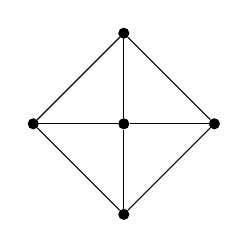
\begin{tikzpicture}[scale=1.15]
        \node[circle, fill, scale=0.015cm] (c) at (0, 0) {};
        \node[circle, fill, scale=0.015cm] (l1) at (1, 0) { };
        \node[circle, fill, scale=0.015cm] (l2) at (0, -1) { };
        \node[circle, fill, scale=0.015cm] (l3) at (-1, 0) {};
        \node[circle, fill, scale=0.015cm] (l4) at (0, 1) {};

        \draw (c) -- (l1);
        \draw (c) -- (l2);
        \draw (c) -- (l3);
        \draw (c) -- (l4);
        \draw (l1) -- (l2) -- (l3) -- (l4) -- (l1);

    \end{tikzpicture}
    \hspace{0.5cm}
    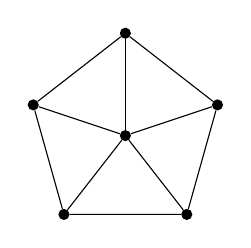
\begin{tikzpicture}[scale=1.3]
        \node[circle, fill, scale=0.015cm] (c) at (0, 0) {};
        \node[circle, fill, scale=0.015cm] (l1) at (0, 1) { };
        \node[circle, fill, scale=0.015cm] (l2) at (0.9, 0.30) { };
        \node[circle, fill, scale=0.015cm] (l3) at (0.6, -0.77) {};
        \node[circle, fill, scale=0.015cm] (l4) at (-0.6, -0.77) {};
        \node[circle, fill, scale=0.015cm] (l5) at (-0.9, 0.30) {};

        \draw (c) -- (l1);
        \draw (c) -- (l2);
        \draw (c) -- (l3);
        \draw (c) -- (l4);
        \draw (c) -- (l5);
        \draw (l1) -- (l2) -- (l3) -- (l4) -- (l5) -- (l1);
    \end{tikzpicture}
    \caption{The 4-star and the 5-star.}
\end{figure}

For the 4-star, we know that the only colorings it allows on the ring are those with three colors or less. Hence

\begin{equation}
    \Phi_0(\text{4-star}) = \{ abab, abac, baca \}.
\end{equation}

However, the set of all ring colorings of $R_4$ also includes the coloring $abcd$.

\begin{equation}
    \Phi(4) = \{ abab, abac, baca, abcd \}.
\end{equation}

Therefore, to prove D-reducibility, we must show that $abcd \in \Phi_n(\text{4-star})$ for some $n$-implying set. In this case we obtain that

\begin{equation}
    \scheme{a,b,c,d}{13a} \compat abcb \quad \text{or} \quad \scheme{a,b,c,d}{13a-} \compat abad.
\end{equation}

Both of these colorings are in $\Phi_0(\text{4-star})$ up to permutation. Therefore

\begin{equation*}
    \Phi_1(\text{4-star}) = \{ abcd \}.
\end{equation*}

Hence $\overline{\Phi}(\text{4-star}) = \Phi(4)$ and we can conclude that the 4-star is D-reducible.

However, the 5-star is unfortunately not D-reducible (this would also prove the four color theorem). The problem can quickly be seen from the fact that any chain on a 4-coloring like $abcad$ implies both a 3-coloring and 4-coloring.

\begin{equation*}
    \scheme{a,b,c,a,d}{35c} \compat abcbd \quad \text{or} \quad \scheme{a,b,c,a,d}{35c-} \compat abcbd.
\end{equation*}

The actual proof involves evaluating many cases, which can be done with a computer.

Next we treat C-reducibility that serves as the final form of reducibility required for the four-color theorem.